\chapter{Semafori}

\section{Introduzione}

\dfn{Semaforo}{Un \newfancyglitter{semaforo} è un tipo di dato astratto\footnote{Opaco, non si sa com'è implementato.}, che assume valori interi ì, $\geq$ 0, su cui si eseguono solo due primitive atomiche: P e V (wait, signal).}

\nt{Una variabile di tipo \fancyglitter{semaphore} è condivisibile da due o più processi.}

\clm{}{}{
	\begin{itemize}
		\item Strumento linguistico di "basso livello" per \fancyglitter{problemi di sincronizzazione}.
		\item Normalmente realizzato a \fancyglitter{livello macchina} per realizzare strumenti di sincronizzazione di "più alto livello".
		\item Disponibile in librerie standard per la realizzazione di programmi concorrenti con linguaggi sequenziali.
	\end{itemize}
}

\cor{P}{
	La P prova ad accedere al semaforo. Quando accede decrementa il contatore di 1.
}

\begin{center}
	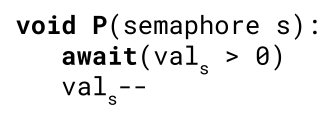
\includegraphics[scale=0.4]{03-Semafori/P.png}
\end{center}

\cor{V}{
	Incremena di 1 il contatore.
}

\begin{center}
	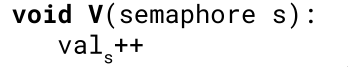
\includegraphics[scale=0.4]{03-Semafori/V.png}
\end{center}

\paragraph{Un semaforo è:}

\begin{itemize}
	\item \fancyglitter{Generalev(o contatore):} se il suo valore può assumere qualsiasi valore intero non negativo.
	\item \fancyglitter{Binario:} se può assumere solo i valori 0 e 1 (la V aumenta solo se il valore corrente è 0).
\end{itemize}

\subsubsection{Implementazione dei Semafori}

La definizione di Dijkstra, essendo astratta, non tiene conto degli aspetti implementativi. Per quanto riguarda l'operazione P sono disponibili varie soluzioni:

\begin{itemize}
	\item \fancyglitter{Busy Waiting:} attesa attiva, \textit{spinlock}.
	\item \fancyglitter{Insieme di processi bloccati}.
	\item \fancyglitter{Coda FIFO di processi bloccati}.
\end{itemize}

\nt{In questo corso non si faranno assunzioni sul tipo di implementazione, ma solamente sulla gestione fair dei processi bloccati.}

\subsection{Invarianti Semaforici}

\dfn{Invariante Semaforico}{
	\begin{itemize}
		\item $I_{sem}$: valore intero $\geq$ 0 con cui il semaforo \newfancyglitter{sem} viene inizializzato.
		\item $NV_{sem}$: numero di volte che l'operazione V(sem) è stata \textit{eseguita} fino allo stato s.
		\item $NP_{sem}$: numero di volte che l'operazione P(sem) è stata \textit{completata} fino allo stato s.

	\end{itemize}

	$$val_{sem}(s) = I_{sem} + NV_{sem}(s) - NP_{sem}(s), \text{ con } val_{sem} \geq 0$$

	In ogni stato vale:

	$$NP_{sem} \leq I_{sem} + NV_{sem}$$

}

\subsubsection{Il Problema della Mutua Esclusione}

Il problema della mutua esclusione tra un insieme di processi si può risolvere con l'utilizzo di un semaforo binario chiamato \fancyglitter{mutex}.

\dfn{Mutex}{
	Il mutex è un semaforo binario inizializzato a 1 con semantica:
	\begin{itemize}
		\item val(mutex) = 1, la sezione critica è libera.
		\item val(mutex) = 0, la sezione critica è stata acquisita da un processi.
	\end{itemize}

	Il \newfancyglitter{prologo} per l'accesso alla CS è costituito dall'operazione P(mutex) e l'\newfancyglitter{epilogo} dall'operazione V(mutex).

}


\begin{center}
	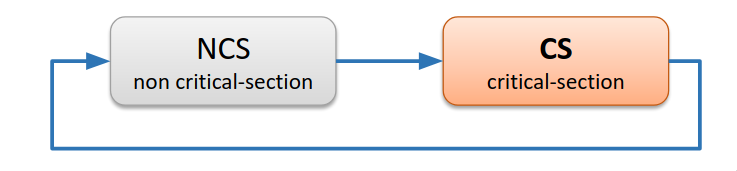
\includegraphics[scale=0.4]{03-Semafori/ME.png}
\end{center}

\paragraph{Una buona soluzione ha:}

\begin{itemize}
	\item \fancyglitter{Mutua Esclusione}.
	\item \fancyglitter{Assenza di Deadlock}.
	\item \fancyglitter{Assenza di Starvation}.
\end{itemize}

\nt{L'assenza di starvation dipende strettamente dall'implementazione dei semafori, quindi si può assumere (ipotesi strong).}

\begin{center}
	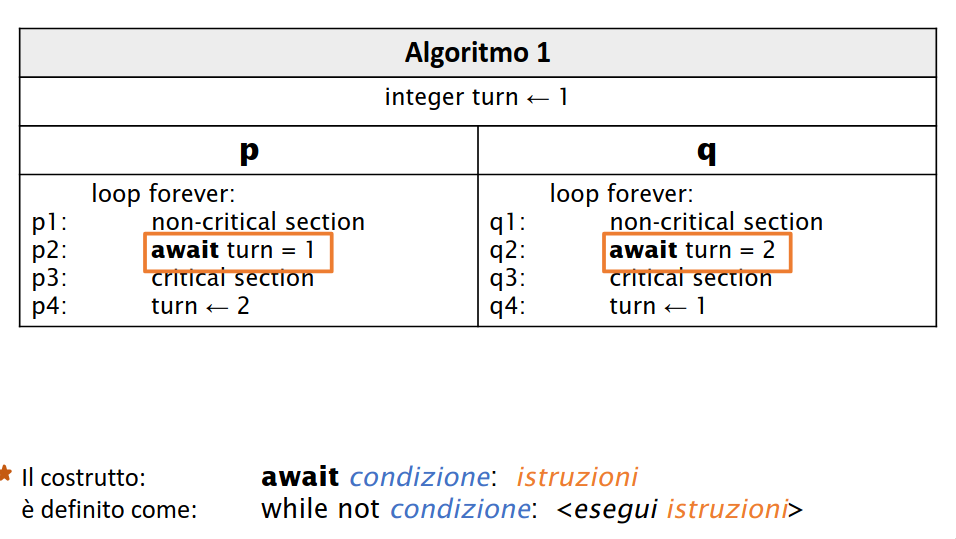
\includegraphics[scale=0.4]{03-Semafori/MEP.png}
\end{center}



\begin{center}
	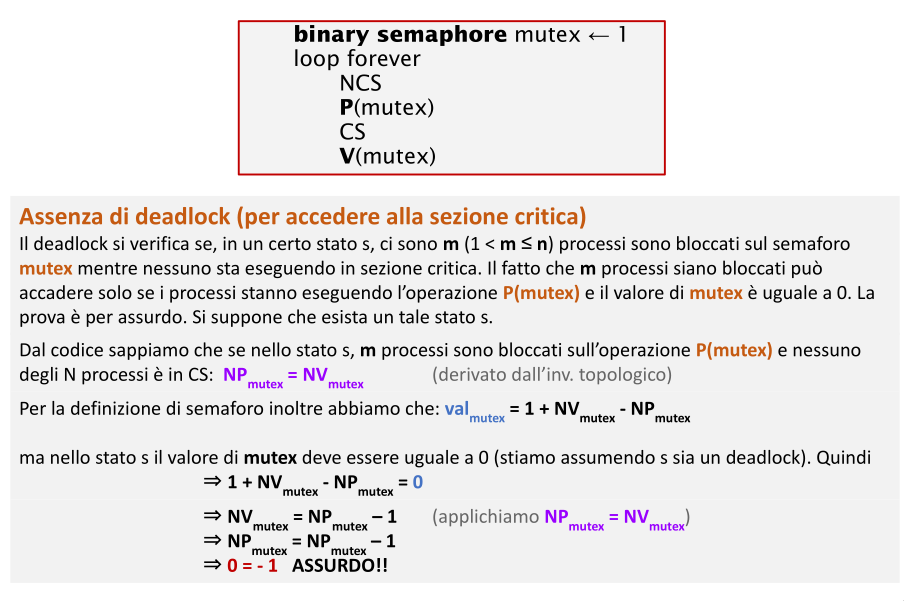
\includegraphics[scale=0.4]{03-Semafori/ADP.png}
\end{center}

\subsection{Semafori per lo Scambio di Segnali Temporali}

Un uso frequente dei semafori è quello di imporre un ordine di esecuzione tra le operazioni dei processi concorrenti.

\begin{center}
	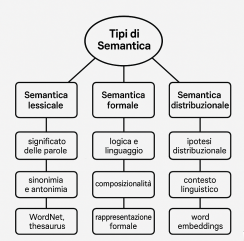
\includegraphics[scale=0.4]{03-Semafori/sem.png}
\end{center}


\dfn{Barriera Sincrona}{
	La \newfancyglitter{barriera sincrona} (o Rendezvous sincrono) tra due processi:

	\begin{itemize}
		\item Due processi P e Q eseguono ciascuno due operazioni consecutive. Pa e Pb il primo, Qa e Qb il secondo.
		\item \newfancyglitter{Vincolo di barriera:} l'esecuzione di Pb da parte di P e quella di qb da parte di Q possono iniziare solo dopo che entrambi i processi hanno completato la loro prima operazione.
	\end{itemize}
}

\begin{center}
	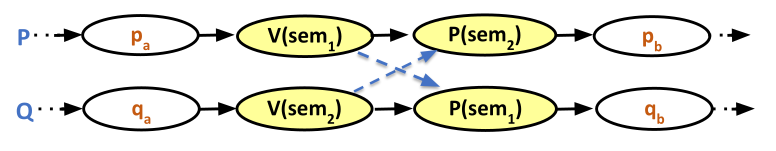
\includegraphics[scale=0.4]{03-Semafori/BS.png}
\end{center}

\subsection{Prove di Correttezza}

\subsubsection{Produttore-Consumatore con un Buffer Infinito}

\begin{itemize}
	\item Due processi, produttore e consumatore, si scambiano dati di tipo \fancyglitter{type} utilizzando un buffer condiviso infinito.
	\item Il consumatore non deve cercare di prelevare un dato dal buffer quando questo è vuoto. Se il consumatore trova il buffer vuoto deve attendere.
	\item Si suppone che \fancyglitter{take} e \fancyglitter{append} siano atomiche.
\end{itemize}

\begin{center}
	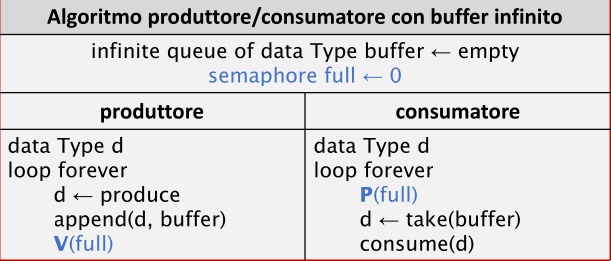
\includegraphics[scale=0.4]{03-Semafori/ProdCons.png}
\end{center}

\subsubsection{Produttore-Consumatore con un Buffer Limitato}

\begin{itemize}
	\item Due processi, produttore e consumatore, si scambiano dati di tipo \fancyglitter{type} utilizzando un buffer condiviso in grado di contenere max dati.
	\item Il consumatore non deve cercare di prelevare un dato dal buffer quando questo è vuoto. Se il consumatore trova il buffer vuoto deve attendere.
	\item Il produttore non deve cercare di inserire un dato nel buffer quando questo è pieno.
	\item Si suppone che \fancyglitter{take} e \fancyglitter{append} siano atomiche.
\end{itemize}

\begin{center}
	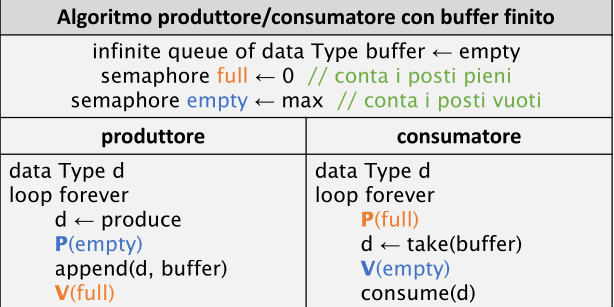
\includegraphics[scale=0.4]{03-Semafori/ProdCons2.png}
\end{center}

\subsubsection{Produttore-Consumatore con un Buffer Circolare}

\begin{center}
	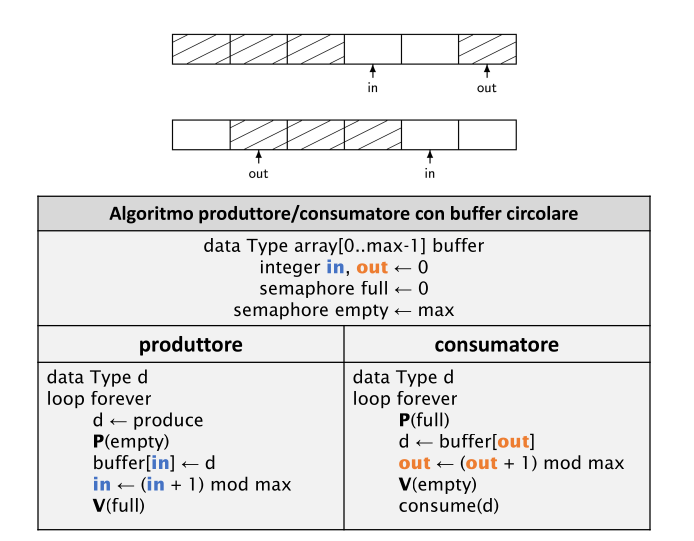
\includegraphics[scale=0.4]{03-Semafori/ProdConsC.png}
\end{center}

\nt{La prova di correttezza è ancora vera se e solo se si assume che ci siano solo un consumatore e un produttore.}

\section{Regione Critica Condizionale}

\begin{itemize}
	\item Può accadere che un'operazione \fancyglitter{op1} richieda di eseguire in sezione
	      critica un codice S1 che necessita della validità di una condizione logica \fancyglitter{C} (precondizione per op1).
	\item Se C non è verificata il processo deve sospendersi e uscire dalla sezione critica.
\end{itemize}

\begin{center}
	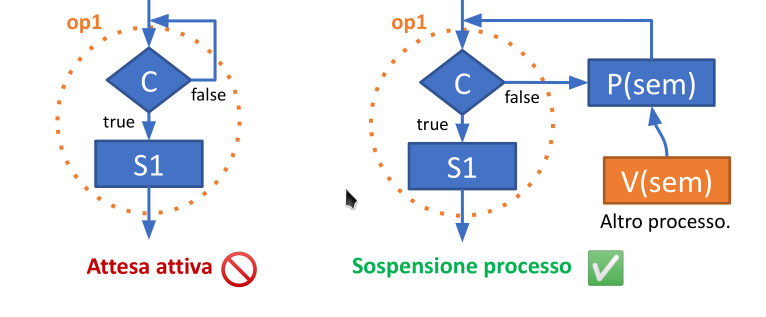
\includegraphics[scale=0.4]{03-Semafori/rc.png}
\end{center}

\paragraph{Condizioni necessarie per realizzare l'attesa:}

\begin{itemize}
	\item Disporre di un semaforo sem, inizializzato a zero, il cui compito è \fancyglitter{bloccare il processo}.
	\item Supporre che sia disponibile un’operazione
	      op2 invocata da un altro processo che
	      modifichi le variabili condivise, in modo che C
	      diventi vera.
	\item Inserire in coda al codice di op2 gli statement
	      opportuni per eseguire il risveglio del processo
	      bloccato sul semaforo sem.
	\item Per sapere se ci sono processi bloccati su sem
	      introduciamo una variabile csem, inizializzata
	      a 0, che memorizza il numero di processi
	      bloccati su sem.
\end{itemize}

\subsection{Tipi di Regione Critica Condizionale}

\begin{center}
	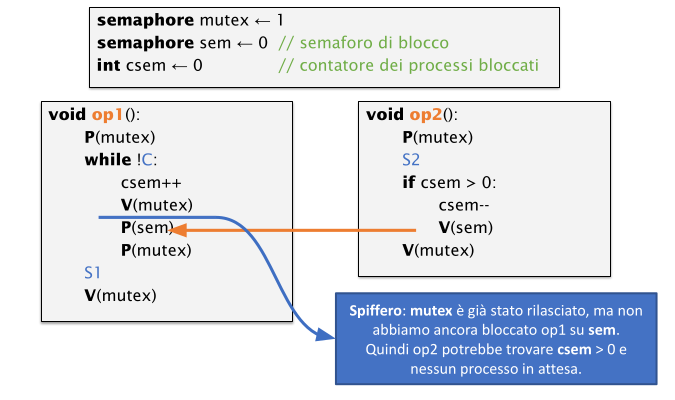
\includegraphics[scale=0.4]{03-Semafori/rcc.png}
\end{center}

\paragraph{Regione critica con attesa circolare:}

\begin{itemize}
	\item Perché quando un processo bloccato sul semaforo
	      sem viene risvegliato e ritorna in CS, ha bisogno di
	      testare nuovamente la condizione C?
	\item È necessario perché l’esecuzione dell’istruzione
	      P(mutex) da parte del processo risvegliato non
	      assicura che il processo possa subito rientrare in CS.
\end{itemize}

\begin{center}
	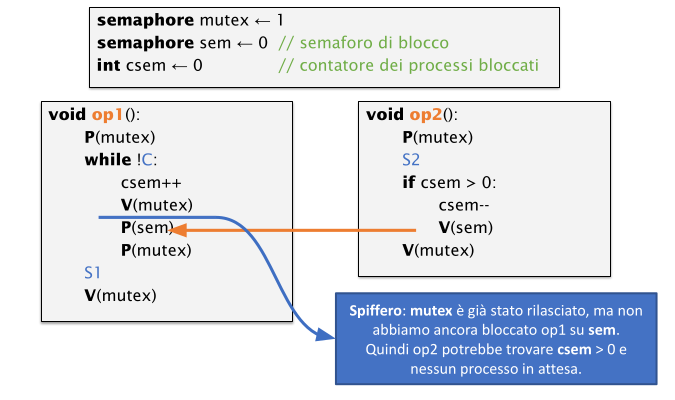
\includegraphics[scale=0.4]{03-Semafori/rcc.png}
\end{center}

\paragraph{Regione critica con passaggio del testimone:}

\begin{itemize}
	\item Nello schema del passaggio del testimone il processo che ha
	      eseguito op2 sveglia il processo bloccato sul semaforo sem senza
	      rilasciare la sezione critica (esecuzione di V(mutex)), così il processo
	      risvegliato trova già la sezione critica bloccata (non deve eseguire
	      P(mutex)) e non serve ritestare la condizione C.
	\item Quindi il processo che termina l’esecuzione di op2 passa al processo
	      svegliato il diritto di operare in CS (da qui il nome di passaggio di
	      testimone).

\end{itemize}

\clm{}{}{
	\begin{itemize}
		\item La regione critica con attesa circolare potrebbe essere sub-ottimale perché
		      richiede al processo di riverificare la validità di C.
		\item Nel caso in cui già sapessimo che C diventa vera dopo S2,
		      stiamo rieseguendo un controllo non necessario.
		\item Tuttavia l'attesa circolare è più generale del passaggio del testimone perché non assume che si debba sapere che la
		      proprietà C sia vera dopo l’esecuzione di S2.
	\end{itemize}
}

\section{Semafori Privati}

\paragraph{Partendo dal problema della regione critica condizionale:}

\begin{itemize}
	\item Più processi possono essere bloccati durante l’esecuzione
	      dell’operazione op1, ciascuno in attesa che la propria condizione di
	      sincronizzazione sia verificata.
	\item In seguito alla modifica dello stato della risorsa condivisa da parte
	      del processo che ha eseguito op2, può accadere che le condizioni di
	      sincronizzazione dei processi bloccati risultino tutte vere.
	\item Se i processi sono bloccati tutti su un semaforo sem, la scelta del
	      processo da svegliare dipende da come è implementata V(sem).
	\item Per cui si deve eseguire una \fancyglitter{politica di risveglio dei
		      processi bloccati}.
	\item Per farlo basta sostituire sem con un array di semafori privati (uno per ciascun processo che può eseguire op1).
\end{itemize}

\subsection{Problema dei Lettori/Scrittori}

Un insieme di processi condivide un database. I processi sono divisi in due gruppi: i \fancyglitter{lettori} e gli \fancyglitter{scrittori}.

\paragraph{Vincoli di accesso al database:}

\begin{itemize}
	\item Gli scrittori accedono al database in mutua esclusione. Quando uno
	      scrittore opera sul database, nessun altro scrittore o lettore può operare.
	\item I lettori possono accedere al database in un numero arbitrario.
\end{itemize}

\paragraph{La priorità viene data per garantire l'alternanza:}

\begin{itemize}
	\item Un lettore non accede al database se uno scrittore sta operando sul
	      database o se ci sono scrittori in attesa.
	\item Quando uno scrittore termina e ci sono lettori in coda, questi lettori
	      possono accedere al database (anche se ci sono altri scrittori in attesa).
	\item Uno scrittore non accede al database se questo è già occupato.
\end{itemize}

\begin{center}
	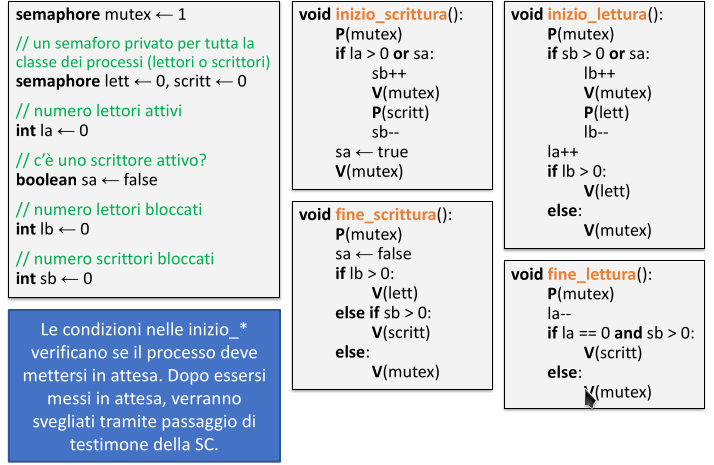
\includegraphics[scale=0.4]{03-Semafori/ls.png}
\end{center}
